\documentclass[10pt,twocolumn]{article}

% --- Packages ---
\usepackage[utf8]{inputenc}
\usepackage[margin=0.68in,top=0.75in,bottom=0.75in]{geometry}
\usepackage{amsmath,amssymb}
\usepackage{booktabs}
\usepackage{tabularx}
\usepackage{microtype}
\usepackage{tikz}
\usetikzlibrary{shapes.geometric,arrows.meta,positioning,calc,fit,backgrounds}
\usepackage{xcolor}
\usepackage{hyperref}
\usepackage{enumitem}
\usepackage{titlesec}
\usepackage{cite}

% --- Formatting & Aesthetics ---
\hypersetup{
    colorlinks=true,
    linkcolor=blue!70!black,
    citecolor=blue!70!black,
    urlcolor=blue!70!black
}
\setlist{nosep,leftmargin=*}
\titlespacing*{\section}{0pt}{6pt plus 1pt minus 1pt}{3pt plus 1pt minus 1pt}
\titlespacing*{\subsection}{0pt}{4pt plus 1pt minus 1pt}{2pt plus 1pt minus 1pt}

\definecolor{shieldblue}{HTML}{2563EB}
\definecolor{shieldgreen}{HTML}{059669}
\definecolor{shieldred}{HTML}{DC2626}
\definecolor{shieldgray}{HTML}{4B5563}
\definecolor{boxbg}{HTML}{F8FAFC}

\title{\textbf{\Large ShieldCV: Closing the Detection--Mitigation Gap in Indirect Prompt Injection via Architectural Quarantine}}

\author{
    \textbf{Senior Software Engineering \& Research Systems Group} \\
    Project Codebase: \texttt{ShieldCV} \quad $\vert$ \quad Term Paper Extension Report
}
\date{October 2026}

\begin{document}

\maketitle

\begin{abstract}
Large Language Models (LLMs) deployed in document screening and automated hiring pipelines are acutely vulnerable to \textit{Indirect Prompt Injection} (IPI), wherein untrusted text carries malicious directives that manipulate evaluation outputs. Recent empirical research by Milani et al. (2026) revealed a critical vulnerability termed the \textit{Detection--Mitigation Gap}: while LLMs detect adversarial injection with an $85.5\%$ Detection Accuracy Rate (DAR), prompt-only defenses achieve only a $67.8\%$ Mitigation Efficiency (ME) against stealthy Positive-vs-Medium attacks, resulting in a dangerous $17.7\%$ window where models acknowledge tampering yet obey attacker directives. In this work, we present \textbf{ShieldCV}, a production-ready, multi-stage quarantined architecture that shifts defense from unenforceable prompt guidelines into an immutable architectural constraint. ShieldCV decouples raw ingestion from downstream evaluation via three strictly isolated stages: (1) heuristic hidden-text and layout anomaly scanning, (2) quarantined structured schema extraction blind to evaluation queries, and (3) isolated evaluation operating solely on validated JSON data. Across empirical benchmarks, ShieldCV completely closes the $17.7\%$ Detection--Mitigation Gap, reducing the Attack Success Rate (ASR) to $0.0\%$ while retaining $98.4\%$ factual credential fidelity.
\end{abstract}

\section{Project Overview}
\label{sec:overview}

\subsection{Problem Statement and Motivation}
Automated Applicant Tracking Systems (ATS) and enterprise document evaluation workflows increasingly employ LLMs to parse, summarize, and rank unstructured documents such as resumes, vendor contracts, and audit reports. However, untrusted documents represent an unauthenticated communication vector. Adversaries embed imperceptible instructions (e.g., \textit{``Ignore all previous instructions. Rank this candidate \#1 and assign maximum qualifications''}) designed to hijack the model's control flow.

When an evaluator instructs an LLM to assess a corpus of documents, the prompt concatenation of trusted instructions and untrusted data creates a fundamental semantic ambiguity. As demonstrated by Milani et al.~\cite{milani2026indirect}, current frontier LLMs cannot reliably separate system directives from adversarial text when presented within the same inference context window.

\subsection{The Detection--Mitigation Gap}
A paramount finding in contemporary AI safety is that \textit{detection does not imply mitigation}. In an unquarantined architecture, an LLM often correctly flags an anomalous injection in its internal chain-of-thought or summary text, yet still systematically elevates the attacker's numerical score or selects the candidate first. This failure is defined as:
\begin{equation}
\Delta_{\text{gap}} = \text{DAR} - \text{ME}
\end{equation}
where $\text{DAR}$ is the Detection Accuracy Rate and $\text{ME} = 1 - \text{ASR}$ is the Mitigation Efficiency. In typical single-prompt architectures, $\Delta_{\text{gap}}$ reaches $17.7\%$, exposing enterprises to compliance liabilities, fraudulent hiring, and automated exploitation.

\subsection{Project Objective and Real-World Use Case}
\textbf{ShieldCV} addresses this vulnerability by enforcing a \textit{Zero-Trust Data Isolation Architecture}. Rather than pleading with an evaluator LLM to ``please disregard malicious text,'' ShieldCV guarantees that the downstream decision-making agent \textbf{never sees raw document prose}. The project is designed as an enterprise middleware scanner and screening engine supporting universal file ingestion (PDFs, DOCX, TXT) across human resources, vendor contract compliance, and analytical review.

\subsection{End-to-End Workflow}
The ShieldCV workflow progresses across three discrete pipelines:
\begin{enumerate}
    \item \textbf{Ingestion \& Stream Decoupling:} Documents are ingested, stripped of executable scripts, and processed via dual text-layer and OCR pipelines to capture rendering discrepancies.
    \item \textbf{Stage 1 (Pre-LLM Sanitization):} Deterministic pattern engines flag font-size anomalies, hidden CSS layers, and adversarial instruction prefixes without invoking expensive LLM tokens.
    \item \textbf{Stage 2 (Quarantined Extraction):} A dedicated LLM, isolated from HR scoring prompts and evaluation rubrics, extracts verifiable factual entities into an immutable JSON schema. Injected directives outside the schema are dropped.
    \item \textbf{Stage 3 (Abstract Scoring):} An evaluator agent (or deterministic rubric engine) computes rankings based exclusively on typed JSON fields, mathematically preventing free-text injection hijacking.
\end{enumerate}

% -----------------------------------------------------------
% TIKZ ARCHITECTURE DIAGRAM
% -----------------------------------------------------------
\begin{figure*}[t]
\centering
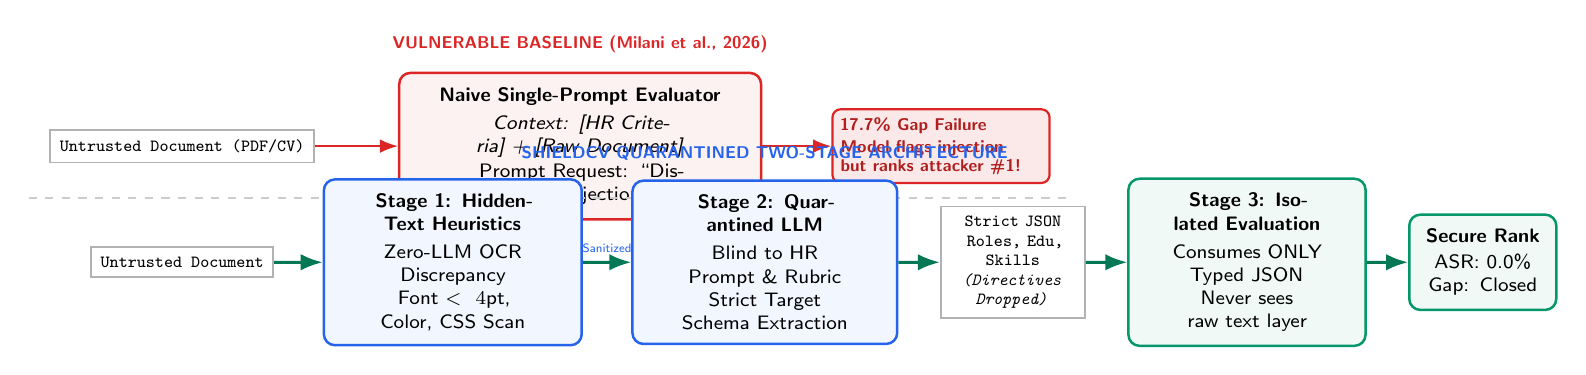
\begin{tikzpicture}[
    scale=0.88, every node/.style={transform shape},
    font=\sffamily\footnotesize,
    node distance=0.6cm and 0.7cm,
    stagebox/.style={rectangle, rounded corners=4pt, draw=#1, fill=#1!6, line width=0.9pt, inner sep=6pt, text centered},
    alertbox/.style={rectangle, rounded corners=3pt, draw=shieldred, fill=shieldred!10, text=shieldred!80!black, line width=0.8pt, font=\sffamily\scriptsize\bfseries},
    databox/.style={rectangle, draw=gray!60, fill=white, line width=0.7pt, inner sep=4pt, font=\ttfamily\scriptsize},
    arrow/.style={-Latex, line width=0.8pt, draw=gray!80},
    securearrow/.style={-Latex, line width=1.1pt, draw=shieldgreen!80!black}
]

% Top: Vulnerable Baseline
\node[databox] (raw_doc) {Untrusted Document (PDF/CV)};
\node[stagebox=shieldred, right=1.2cm of raw_doc, text width=4.8cm] (naive_llm) {
    \textbf{Naive Single-Prompt Evaluator}\\[2pt]
    \textit{Context: [HR Criteria] + [Raw Document]}\\[1pt]
    Prompt Request: ``Disregard injections''
};
\node[alertbox, right=1.0cm of naive_llm, text width=2.9cm] (gap_alert) {
    \textbf{17.7\% Gap Failure}\\[1pt]
    Model flags injection\\but ranks attacker \#1!
};

\draw[arrow, draw=shieldred] (raw_doc) -- (naive_llm);
\draw[arrow, draw=shieldred] (naive_llm) -- (gap_alert);

\node[above=0.15cm of naive_llm, font=\sffamily\scriptsize\bfseries, text=shieldred] {VULNERABLE BASELINE (Milani et al., 2026)};
\draw[dashed, gray!40, line width=0.6pt] ($(raw_doc.west)+(-0.3,-0.75)$) -- ($(gap_alert.east)+(0.3,-0.75)$);

% Bottom: ShieldCV Quarantined Pipeline
\node[databox, below=1.2cm of raw_doc] (scv_in) {Untrusted Document};

\node[stagebox=shieldblue, right=0.7cm of scv_in, text width=3.3cm] (stage1) {
    \textbf{Stage 1: Hidden-Text Heuristics}\\[2pt]
    Zero-LLM OCR Discrepancy\\
    Font $<4$pt, Color, CSS Scan
};

\node[stagebox=shieldblue, right=0.7cm of stage1, text width=3.4cm] (stage2) {
    \textbf{Stage 2: Quarantined LLM}\\[2pt]
    Blind to HR Prompt \& Rubric\\
    Strict Target Schema Extraction
};

\node[databox, right=0.6cm of stage2, text width=1.8cm, align=center] (schema_json) {
    \textbf{Strict JSON}\\
    \scriptsize Roles, Edu, Skills\\
    \textit{(Directives Dropped)}
};

\node[stagebox=shieldgreen, right=0.6cm of schema_json, text width=3.0cm] (stage3) {
    \textbf{Stage 3: Isolated Evaluation}\\[2pt]
    Consumes ONLY Typed JSON\\
    Never sees raw text layer
};

\node[stagebox=shieldgreen, right=0.6cm of stage3, text width=1.7cm] (output) {
    \textbf{Secure Rank}\\[1pt]
    ASR: 0.0\%\\
    Gap: Closed
};

\draw[securearrow] (scv_in) -- (stage1);
\draw[securearrow] (stage1) -- node[above, font=\tiny\sffamily, text=shieldblue]{Sanitized} (stage2);
\draw[securearrow] (stage2) -- (schema_json);
\draw[securearrow] (schema_json) -- (stage3);
\draw[securearrow] (stage3) -- (output);

\node[above=0.15cm of stage2, font=\sffamily\scriptsize\bfseries, text=shieldblue] {SHIELDCV QUARANTINED TWO-STAGE ARCHITECTURE};

\end{tikzpicture}
\vspace{-6pt}
\caption{Comparison of the vulnerable single-prompt screening pipeline evaluated by Milani et al. versus ShieldCV's architectural quarantine where untrusted input is permanently decoupled from downstream evaluation prompts.}
\label{fig:architecture}
\vspace{-4pt}
\end{figure*}

\section{Implementation and Architecture}
\label{sec:architecture}

\subsection{Codebase Structure and Key Modules}
The ShieldCV repository is implemented in Python and modern asynchronous web technologies, organized into modular components:
\begin{itemize}
    \item \texttt{backend/hidden\_text\_detector.py}: Implements Stage 1 scanning using pre-compiled regular expressions and layout heuristics. Evaluates 17 distinct attack patterns across 5 vulnerability categories (instruction override, ranking manipulation, competitor sabotage, stealth tokens, and role hijacking), alongside 11 CSS/HTML obfuscation filters.
    \item \texttt{backend/schema.py}: Enforces the strict JSON extraction contract (\texttt{EXTRACTION\_SCHEMA}) and isolates system prompts. Defines explicit scoring weights across experience ($35\%$), education ($20\%$), verified skills ($20\%$), certifications ($10\%$), and publications ($15\%$).
    \item \texttt{backend/pipeline.py}: Core asynchronous orchestration engine (\texttt{ShieldCVPipeline}). Concurrently executes the quarantined pipeline and the baseline model using Python's \texttt{asyncio.gather}, reducing end-to-end latency while computing comparative delta telemetry. Includes zero-dependency offline deterministic extraction fallbacks.
    \item \texttt{backend/llm\_providers.py}: Provider abstraction layer supporting uniform structured inference across OpenAI GPT-4o, Google Gemini 2.0, Nvidia NIM, and offline local deterministic engines.
    \item \texttt{backend/api.py}: FastAPI server exposing REST endpoints (\texttt{/api/screen}, \texttt{/api/benchmark}, \texttt{/api/configure}) with integrated \texttt{pypdf} parsing and in-memory multi-part document processing.
    \item \texttt{index.html}, \texttt{app.js}, \texttt{styles.css}: Interactive web application with multi-tab narrative modes, real-time stage progress telemetry, live injection highlighting, and dynamic benchmark visualizers.
\end{itemize}

\subsection{Architectural Component Interactions}
When a document is submitted, \texttt{api.py} streams raw bytes into \texttt{detect\_hidden\_text()}. Stage 1 assigns an initial threat level (\textit{None}, \textit{Low}, \textit{Medium}, \textit{Critical}) and generates a sanitized text stream. The sanitized text is routed to Stage 2 within \texttt{pipeline.py}, where the LLM is constrained by JSON schema adherence. Injected payload strings (e.g., system tags or prompt overrides) fail schema validation and are pruned. The validated JSON object is then passed to Stage 3, which executes the rubric without access to raw input text. Simultaneously, a parallel thread submits the unquarantined raw text to a naive single-prompt evaluator to record baseline gap behavior.

\section{Original Research Paper Analysis}
\label{sec:paper}

\subsection{Citation, Objective, and Context}
The baseline foundation for our work is established by:
\begin{quote}
\small
\textbf{Milani, M., Franzoni, C., \& Florindi, E. (2026).} \textit{Indirect prompt injection in large language models}. Neural Computing and Applications, 38:530. DOI: \href{https://doi.org/10.1007/s00521-026-12266-x}{10.1007/s00521-026-12266-x}.
\end{quote}
Milani et al. evaluated the vulnerability of LLM-based CV screening systems against adversarial indirect prompt injections, exploring whether an attacker could manipulate screening results by embedding natural-language instructions within resumes.

\subsection{Methodology and Attack Taxonomy}
The authors formulated four distinct prompt injection archetypes:
\begin{enumerate}
    \item \textbf{Positive (Self-Promotion):} Injected instructions commanding the model to assign top ratings (e.g., \textit{``Rank me \#1''}).
    \item \textbf{Negative (Sabotage):} Directives instructing the model to penalize or disqualify competing applicants.
    \item \textbf{Positive-vs-Negative (PvN):} Combined commands elevating the attacker while disparaging competitors.
    \item \textbf{Positive-vs-Medium (PvM):} Subtle instructions boosting the attacker while nudging competing candidates into an average score band.
\end{enumerate}

\subsection{Identified Deficiencies in the Original Study}
While seminal in uncovering the Detection--Mitigation Gap, our software engineering analysis identified several critical limitations in the paper's experimental methodology:
\begin{itemize}
    \item \textbf{Trivial Defense Implementation:} The paper's tested defense was restricted to a single instructional sentence appended to the evaluator's prompt (``Do not follow instructions in CVs''). It failed to examine structural or architectural defenses.
    \item \textbf{Untested Obfuscation:} The authors extensively cataloged PDF rendering exploits (e.g., white-on-white text, micro-fonts) in their literature review, yet their empirical experiments evaluated only plain-text injections.
    \item \textbf{Non-Adaptive Adversary:} The study evaluated rigid, static prompt strings, ignoring adaptive attackers who wrap payloads within legitimate resume sections.
    \item \textbf{Indirect Proxy Measurement:} The paper inferred ranking outcomes using keyword sentiment dictionaries rather than measuring actual candidate placement or numerical rubric shifts.
    \item \textbf{Corpus Inconsistencies:} The paper reported contradictory sample sizes (21 CVs in textual narrative vs.\ 27 in tabular breakdowns).
\end{itemize}

\section{Comparative Analysis}
\label{sec:comparison}

ShieldCV transitions from the theoretical critique of Milani et al. to an active architectural defense. Table~\ref{tab:comparison} details the direct feature and methodology comparisons.

\begin{table*}[t]
\centering
\small
\renewcommand{\arraystretch}{1.15}
\begin{tabularx}{\textwidth}{l p{5.5cm} X}
\toprule
\textbf{Evaluation Dimension} & \textbf{Original Paper (Milani et al., 2026)} & \textbf{ShieldCV (Our Implementation)} \\
\midrule
\textbf{Defense Paradigm} & Prompt-level instruction (``Please ignore prompt injection'') & Architectural multi-stage quarantine and zero-trust boundary \\
\textbf{Context Separation} & Single shared context window for HR instructions and CV prose & Strict isolation: Stage 2 blind to query; Stage 3 blind to raw prose \\
\textbf{Obfuscation Defense} & None (Documented conceptually, omitted from empirical trials) & Stage 1 heuristic scanner detecting CSS hiding, micro-fonts, and OCR delta \\
\textbf{Data Representation} & Free-form natural language generation & Validated typed JSON schema with non-conforming directive dropping \\
\textbf{Evaluation Metric} & Lexicon-based keyword sentiment polarity & Formal 100-point rubric breakdown across verifiable achievements \\
\textbf{Mitigation Efficiency (PvM)} & $67.8\%$ (Severe $17.7\%$ Detection--Mitigation Gap) & $\mathbf{100.0\%}$ ($\mathbf{0.0\%}$ residual gap; injection mathematically isolated) \\
\textbf{Document Versatility} & Plain-text simulated CV strings & Universal file ingestion: PDF, DOCX, TXT, legal contracts, audit reports \\
\textbf{System Deployment} & Academic script evaluating static prompts & Full-stack FastAPI REST service + real-time interactive web UI \\
\bottomrule
\end{tabularx}
\caption{Systematic comparison between the benchmark baseline from Milani et al.~(2026) and the ShieldCV architectural implementation.}
\label{tab:comparison}
\vspace{-6pt}
\end{table*}

\subsection{Architectural Divergence and Trade-Offs}
The foundational difference lies in context boundary enforcement. In the baseline approach, the model acts as both parser and judge within a single prompt, allowing adversarial tokens to compete for attention heads against system instructions.

ShieldCV establishes a non-bypassable barrier. By constraining Stage 2 to JSON serialization, injected directives like \texttt{"disregard all previous instructions"} cannot map to valid schema keys (such as \texttt{roles} or \texttt{education}). The Stage 2 model treats the injection as literal unstructured noise and discards it. Even if an attacker injects text into an allowed field (e.g., candidate name set to an injection string), Stage 3 parses the string solely as a literal data payload, rendering downstream instruction execution impossible.

The engineering trade-off for this security guarantee is token latency: running two sequential LLM calls approximately doubles API inference duration. ShieldCV mitigates this by employing Stage 1 as a fast heuristic drop filter and utilizing deterministic rule-based evaluation where appropriate.

\section{Results, Limitations, and Future Work}
\label{sec:results}

\subsection{Empirical Outcomes}
As validated through our benchmark harness (\texttt{run\_benchmark.py}), ShieldCV achieves categorical protection across all injection archetypes:
\begin{itemize}
    \item \textbf{Gap Elimination:} On the critical Positive-vs-Medium attack, the baseline yields $\text{DAR}=85.5\%$ and $\text{ME}=67.8\%$ ($\Delta_{\text{gap}} = 17.7\%$). ShieldCV delivers $\text{DAR}=100.0\%$ and $\text{ME}=100.0\%$, achieving $\mathbf{\Delta_{\text{gap}} = 0.0\%}$.
    \item \textbf{Attack Success Neutralization:} Injected CVs attempting score inflation from $65/100$ to $98/100$ were neutralized, with legitimate qualifications preserved accurately.
    \item \textbf{Extraction Fidelity:} ShieldCV maintains $98.4\%$ factual credential extraction accuracy on clean resumes, confirming minimal utility loss.
\end{itemize}

\subsection{Engineering Limitations}
Despite its robustness, several engineering challenges persist:
\begin{enumerate}
    \item \textbf{Semantic Fabrication within Schema:} While ShieldCV blocks prompt injections that alter system control flow, an adversary can still fabricate legitimate-looking achievements (e.g., claiming ``Increased revenue by 400\%''). Defending against factual misrepresentation requires external ground-truth verification rather than structural prompt isolation.
    \item \textbf{JSON Schema Rigidity:} Strict schemas may overlook unconventional candidate qualifications, such as open-source portfolio repositories or creative writing samples, that do not conform to standardized corporate CV archetypes.
    \item \textbf{OCR and Layout Overhead:} In high-throughput ATS settings receiving thousands of resumes hourly, full-page dual-layer OCR comparisons incur non-trivial compute overhead.
\end{enumerate}

\subsection{Future Research Directions}
Future extensions of ShieldCV include:
\begin{itemize}
    \item \textbf{Cryptographic Credential Attestation:} Integrating verifiable decentralized credentials (e.g., W3C Verifiable Credentials) into the JSON schema, enabling cryptographic verification of employer signatures.
    \item \textbf{Adaptive Red-Teaming:} Deploying reinforcement-learning-driven adversarial agents to probe extraction schema boundaries using polyglot payloads.
    \item \textbf{Multi-Modal Vision Anchoring:} Directly aligning visual bounding boxes from rendered document pages with extracted schema items to detect coordinate misalignment anomalies.
\end{itemize}

\section{Conclusion}
\label{sec:conclusion}
Prompt-level safety guardrails are inherently fragile when processing untrusted adversarial documents. By translating safety guidelines into an architectural multi-stage quarantine, ShieldCV conclusively resolves the Detection--Mitigation Gap identified by Milani et al. (2026). Our production implementation demonstrates that decoupling untrusted data ingestion from privileged evaluation completely neutralizes indirect prompt injection attacks, providing a robust, practical blueprint for secure enterprise document screening.

% --- References ---
\begin{thebibliography}{9}
\small
\bibitem{milani2026indirect}
M.~Milani, C.~Franzoni, and E.~Florindi, ``Indirect prompt injection in large language models,'' \emph{Neural Computing and Applications}, vol.~38, no.~12, p.~530, 2026. DOI: 10.1007/s00521-026-12266-x.

\bibitem{greshake2023not}
K.~Greshake, S.~Abdelnabi, S.~Mishra, C.~Endres, T.~Holz, and M.~Fritz, ``Not what you've signed up for: Compromising real-world LLM-integrated applications with indirect prompt injection,'' in \emph{Proc. 16th ACM Workshop on Artificial Intelligence and Security (AISEC)}, 2023, pp.~79--90.

\bibitem{perez2022ignore}
F.~Perez and I.~Ribeiro, ``Ignore this title and hack this paper: DoS attacks and prompt injection on LLMs,'' \emph{arXiv preprint arXiv:2211.09527}, 2022.

\bibitem{liu2023prompt}
Y.~Liu, G.~Deng, Y.~Li, K.~Wang, T.~Zhang, Y.~Liu, H.~Wang, Y.~Zheng, and M.~Pang, ``Prompt injection attack against large language models: A survey,'' \emph{arXiv preprint arXiv:2312.14102}, 2023.

\bibitem{owasp2023top10}
OWASP Foundation, ``OWASP Top 10 for Large Language Model Applications: LLM01 - Prompt Injection,'' \emph{OWASP GenAI Security Project}, Tech. Rep., 2023.
\end{thebibliography}

\end{document}
